\documentclass[main]{subfiles} 
\graphicspath{{img/}}


\begin{document}

\section{Methodology}
A big difference between real estate and other publicly traded assets is that there is no centralized platform where offers can be tracked. 
In the case of asset classes such as bonds and equity this service is provided by multiple sources such as Bloomberg, Refinitiv and Morningstar.

Something similar is missing for the Swiss real estate market. 
Usually real estate on the various websites is presented as a list of single "tiles", 
along with a brief overview of the key data of the corresponding property (for reference see figure \ref{fig:listing}).
Normally there is no possibility to see the average cost per square meter in the ZIP code 
and no real way to compare similar estates.

Given that the data is neither available via an \acs*{api} nor through an already established database,
the decision was made to write an algorithm that scrapes the required data from a website.


\subsection{Choice of Website}

Whilst there exist numerous websites that act as middlemen between buyer and seller such as \verb|www.immoscout24.ch| and \verb|www.homegate.ch|,
all of them suffer from the same underlying problem mentioned in the introduction. 
Selecting and pricing real estate by clicking through listing after listing is cumbersome and inefficient.
Furthermore, with the data being split up over many websites, a buyer might not find his ideal new property, simply by looking on the wrong platform.

An attempt at creating a more transparent and efficient real estate market was made by Comparis. 
On their website, listings from many sources are aggregated and displayed according to their key characteristics.
However, also \verb|www.comparis.ch| does not offer tools for further analysis and does not readily display historical data,
except for increases or decreases in the price in percentage.

For the purpose of creating a database which provides a user with information on as many properties in a given area as possible, 
\verb|www.comparis.ch| is the ideal target for scraping data.


\subsection{Web Scraper}

When creating a web scraping application in Python, there are a number of packages and tools to choose from.
These modules include, but are not limited to Requests, Beautifulsoup, Scrapy and last but not least, Selenium.
Each come with their advantages and disadvantages. 
The former two modules, Requests and Beautifulsoup, both come with the bonus of ease of use.
The latter two modules offer more functionality, but have a steeper learning curve.

After several attempts, the choice was made to use a combination of selenium and scrapy.
This decision was based on the need to not only collect data that can be seen on any listing (see \ref{fig:listing}) 
\begin{figure}[htbp]
    \centerline{
        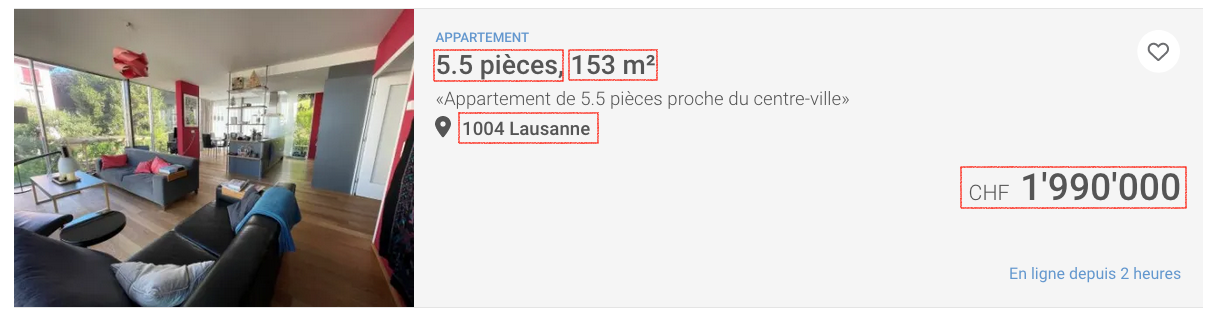
\includegraphics[width = 92mm]{prog_1.png}}
    \caption{Typical Listing on Comparis}
    \label{fig:listing}
\end{figure}

With the objective of creating a platform that includes information on properties in greater Lausanne, 
it became clear that data beyond the filing was needed.


\subsubsection{Selenium}
Selenium allows a user to control any browser environment, provided the corresponding driver has been installed.
Controlling a browser offers several advantages 

\subsubsection{Scrapy}




\subsection{User platform}
To make the dataset scrapped from immoscout more user friendly we decided to build a graphical user interface(GUI).
This way the user will be able to search for a property within a certain price range, zip code or with specific features, 
instead or having to go through the full scrapped dataset.\par
We used the open source library tkinter to model the GUI. We chose this library as it is pre installed in python.
Moreover it is stable and flexible and provides simple syntax.\par
Tkinter is the perfect tool for this first prototype. However, if the project grows tkinter will not be powerful enough,
therefore we recommend switching to PyQT another UI or even REACT for a more professional look. 


\subsection{Structure}


\end{document}